\section{Interfaces}
In this section, we specify interfaces for all objects in the software model, as seen in figure \ref{fig:softwareArchitecture}. This includes the sensor controllers, which are intended to abstract from hardware specific information like the calibration of sensors and filtering out incorrect measurements from the raw data. 

\subsection{Sensor Controllers}
The sensor controller classes all require a calibrate-method, which is called whenever the bus starts, in order to ensure the sensors and motors work as intended. Inheritance is utilised to show this similarity between the individual Sensor Controllers. See figure \ref{fig:interfaceSensorControllers} for a class diagram showing the hierarchy, functions and properties of the Sensor Controllers. Note that constructors and destructors are omitted from this, as they provide little insight to the functionality of the classes. 

\subsection{SensorControllers}
See figure \ref{fig:interfaceSensorControllers} 

\begin{figure}[ht]
    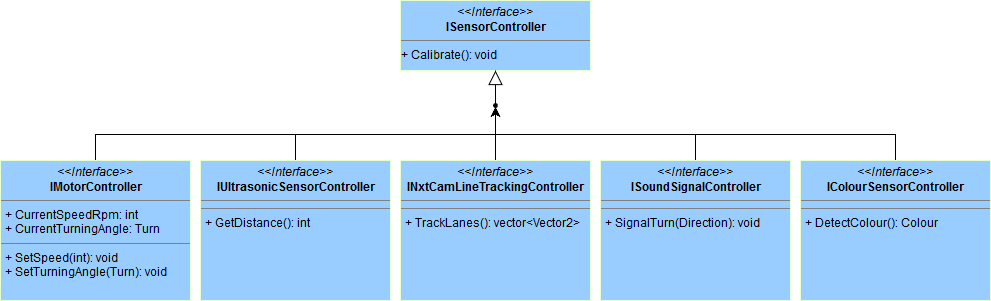
\includegraphics[width=\textwidth]{Images/Design/InterfaceSensorControllers.png}
    \caption{Class diagram showing the sensor controller interfaces}
    \label{fig:interfaceSensorControllers}
\end{figure}

\code{Turn} is a class containing the degrees of the specified turn that is to be executed. \code{Direction} and \code{Colour} are both enumeration types that contain a number of associated options (e.g. left or right, or different colours). Rpm from \code{CurrentSpeedRpm} abbreviates rotations per minute.

\subsection{Components}
The components call the sensor controllers in order to obtain the necessary sensor measurements, and also call the calibration of their corresponding sensors. See figure \ref{fig:interfaceComponents} for a class diagram describing the planned interface structure.

\begin{figure}[ht]
    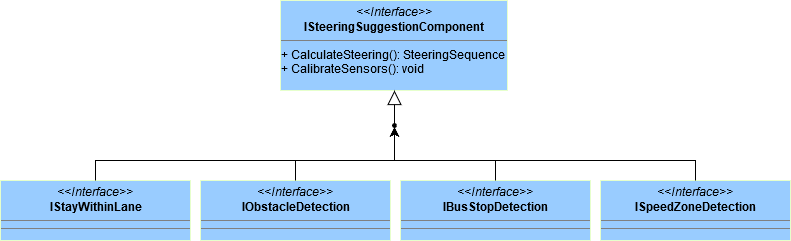
\includegraphics[width=\textwidth]{Images/Design/InterfaceComponents.png}
    \caption{Class diagram showing the component interfaces\todo[inline]{From supervisor: It is very nice to have a unified interface to each piece of code -- it should help to formalize the tasks for scheduling.
So the top interface is very usefull, but the lower ones are interfaces too?
Do you expect a class diagram to continue down below the inheritance hierarchy?}}
    \label{fig:interfaceComponents}
\end{figure}

All components have their \code{CalculateSteering}-method called by the \code{Driving}-component, to which they then return the \code{SteeringSequence} that they suggest the bus should drive. Based on the values it gets, the \code{Driving}-component later decides how to actually drive. 

The class \code{SteeringSequence} contains one or multiple \code{SteeringCommands}, which contains a distance, speed and a \code{Turn} that the bus should drive. Multiple \code{SteeringCommands} can be used for things like braking the bus smoothly through multiple steps, or stopping at a bus stop and other similar manoeuvres. 



\todo{This has changed, so change the diagram: remove the ISteeringSuggestionComponent superclass, remove calibration and add the different return values below. Similarly, the entirety of the design chapter has a few outdated diagrams, which need to be fixed.}

%Right now it's planned the following way: Every time we start executing a new command we note how much distance that command wants to cover (fx. drive 50km/hr for 30 meters). Then, every time steer is called, we start a new command only if the current command is finished. If the SteeringSequence is still at the top of the queue, we move on with the next command in the sequence, and if it's not then we do the other SteeringCommand, then later we continue the Sequence.

%Maybe we need to give the components information about what they signalled last time? They should keep that info themselves, if necessary. 

\subsection{Driving}
\code{Driving} is the class that couples the system together as a supervisory control. As such, it initialises the classes (calibrating the sensors at the same time), calls the components and decides how to steer the bus. See figure \ref{fig:interfaceDriving} for the interface of the \code{Driving} class.

\begin{figure}[ht]
\begin{centering}
    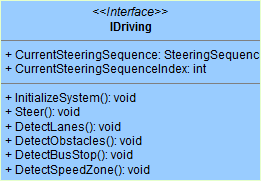
\includegraphics[scale=0.8]{Images/Design/interfaceDriving.png}
    \caption{Interface of the driving class}
    \label{fig:interfaceDriving}
    \end{centering}
\end{figure}



\todo{Write the following comment in english to cap off the section:}
%I programmet bruger vi ikke rent faktiske interfaces af to grunde. Først og fremmest programmerer vi i C++, der ikke giver elegant understøttelse af interfaces. Derudover laver vi et realtidssystem, og da der ikke direkte er noget krav for klar modularitet og udskiftelige komponenter, så er det så at sige en unødvendig brug af den begrænsede hukommelse vi har på Nxt'en.